
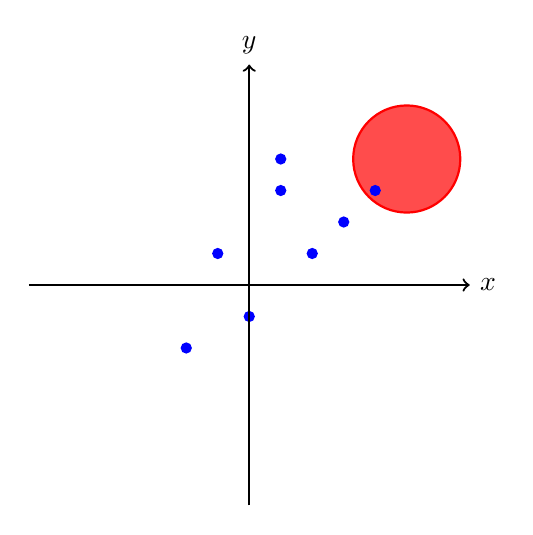
\begin{tikzpicture}[thick, scale=0.4,dot/.style={fill=blue,circle,minimum size=1pt}]




%\filldraw [fill=orange!10,draw=orange,thick] (0,1) circle (5.4);

%\filldraw [fill=yellow!70,draw=yellow,thick] (0,1) circle (3);
%\filldraw [fill=green!10,draw=green,thick]
%(-2.3, -3.3) rectangle (4.5, 4.5);
\filldraw [fill=red!70,draw=red,thick] (5,4) circle (1.70);



\filldraw [blue] (-1,1) circle (4pt)
(1,3) circle  (4pt)
(3,2) circle (4pt)
(4,3) circle (4pt)
(1,3) circle (4pt)
(1,4) circle (4pt)
(0,-1) circle (4pt)
%(2,-3) circle (4pt)
(2,1) circle (4pt)
(-2,-2) circle (4pt);
\draw[->, thick] (-7,0)--(7,0) node[right]{$x$};
\draw[->, thick] (0,-7)--(0,7) node[above]{$y$};


\end{tikzpicture}
